\section{Proposed Research}

In this section, I propose the research I intend to perform. I begin by justifying why a Bayesian approach is not appropriate, but ideal.  I then go on to describe the models I intend to construct.  Finally, I explain how these models will be used to learn about the patient's metabolism in an optimal fashion, and how I will use those models to make optimal doses.

\subsection{Justification for Adopting a Bayesian Framework}

The Bayesian framework is not as computationally simple as the Frequentist framework.  Good justification is required for adopting a Bayesian perspective on Apixiban pharmacokinetics, especially in light of Frequentist non-linear mixed effect models for ODEs \cite{tornoe2004non}.  Here, I discuss just some benefits of adopting a Bayesian framework over a Frequentist framework.

In the proposed application, new patient's pharamcokinetic parameters will be estimated from the model with as few as one measurement per patient.  Estimating several parameters from a single observation in a mixed effects model presents statistical obstacles which are difficult to overcome.  In a Bayesian framework, the prior distribution can make estimating these parameters from sparse data possible.  Of course, this relies on an informative prior.  However, my partnership with clinical pharmacologists will provide rich pharmacological experience to the project, which can then be translated into appropriate and informative priors.  Moreover, the asymptotic arguments used to develop tests of hypothesis in Frequentism may not be valid in application because sample sizes are so small.  Adopting a Bayesian framework will allow for explicit modelling of uncertainty propagation without assuming that asymptotics are valid.

Finally, sequential decision making plays a central role in the proposed research \'{a} la reinforcement learning.  Since posteriors from previous experiments can be used as priors for future experiments, Bayesianism provides a natural framework for sequential evaluation of evidence and decision support.


\subsection{Bayesian Pharmacokinetic Models}

The construction of appropriate Bayesian models for application is non-trivial.  Great care should be taken to construct a model which is sufficiently complex to capture relevant features of the phenomenon, but not so complex as to over fit on the data. 

 The line between appropriately complex and overfit models is not easy to discern.  A recommended strategy for constructing Bayesian models is to start simple, essentially from a model which is ostensibly wrong, and slowly build in complexity, checking the model's implications and improving the model where needed.  Gelman calls this process ``continuous model expansion" \cite{gelman2013bayesian, gelman2013philosophy}.  For the proposed research, a very simple Bayesian model of Apixiban pharmacokinetics will be proposed.  Several expanded models will also be considered and further expanded where needed. Models will be assessed by checking for patterns in the residuals as well as posterior predictive checks.

Data from a controlled experiment \cite{tirona2018apixaban} will be used as a ``development set''.  The data contain 36 patients observed over 12 hours. Each subject ingested 2.5 mg of Apixiban and 100 ml of water in a fasted state. Apixiban blood plasma concentrations were recorded, as well as subject covariates.  See \cref{devsettable} for a summary of patients involved.

\begin{table}[t!]
	\centering
\begin{tabular}{lrrrr}
	\toprule
	\multicolumn{1}{c}{ } & \multicolumn{2}{c}{Female} & \multicolumn{2}{c}{Male} \\
	\cmidrule(l{2pt}r{2pt}){2-3} \cmidrule(l{2pt}r{2pt}){4-5}
	& \multicolumn{1}{c}{Control } & \multicolumn{1}{c}{ NAFLD}  & \multicolumn{1}{c}{ Control}  & \multicolumn{1}{c}{NAFLD } \\
	\midrule
	N & 10 & 13 & 2 & 11\\
	Age  & 46.40 (9.13) & 50.62 (13.24) & 57.00 (18.38) & 50.73 (10.96)\\
	Weight (kg)& 85.77 (27.70) & 83.76 (20.93) & 74.60 (17.82) & 97.56 (25.74)\\
	Creatinine ($\mu$M)& 65.70 (10.34) & 70.62 (13.36) & 86.50 (12.02) & 63.73 (10.76)\\
	\bottomrule
\end{tabular}

\caption[Summary of development data set]{Covariate summary for patients in development set \cite{tirona2018apixaban}.  Shown are sample means with sample standard deviations in parentheses.  Data is stratified by sex and group status (patients with and without non-alcoholic fatty liver disease (NAFLD)).}
\label{devsettable}

\end{table}

\begin{figure}[t!]
	\centering
	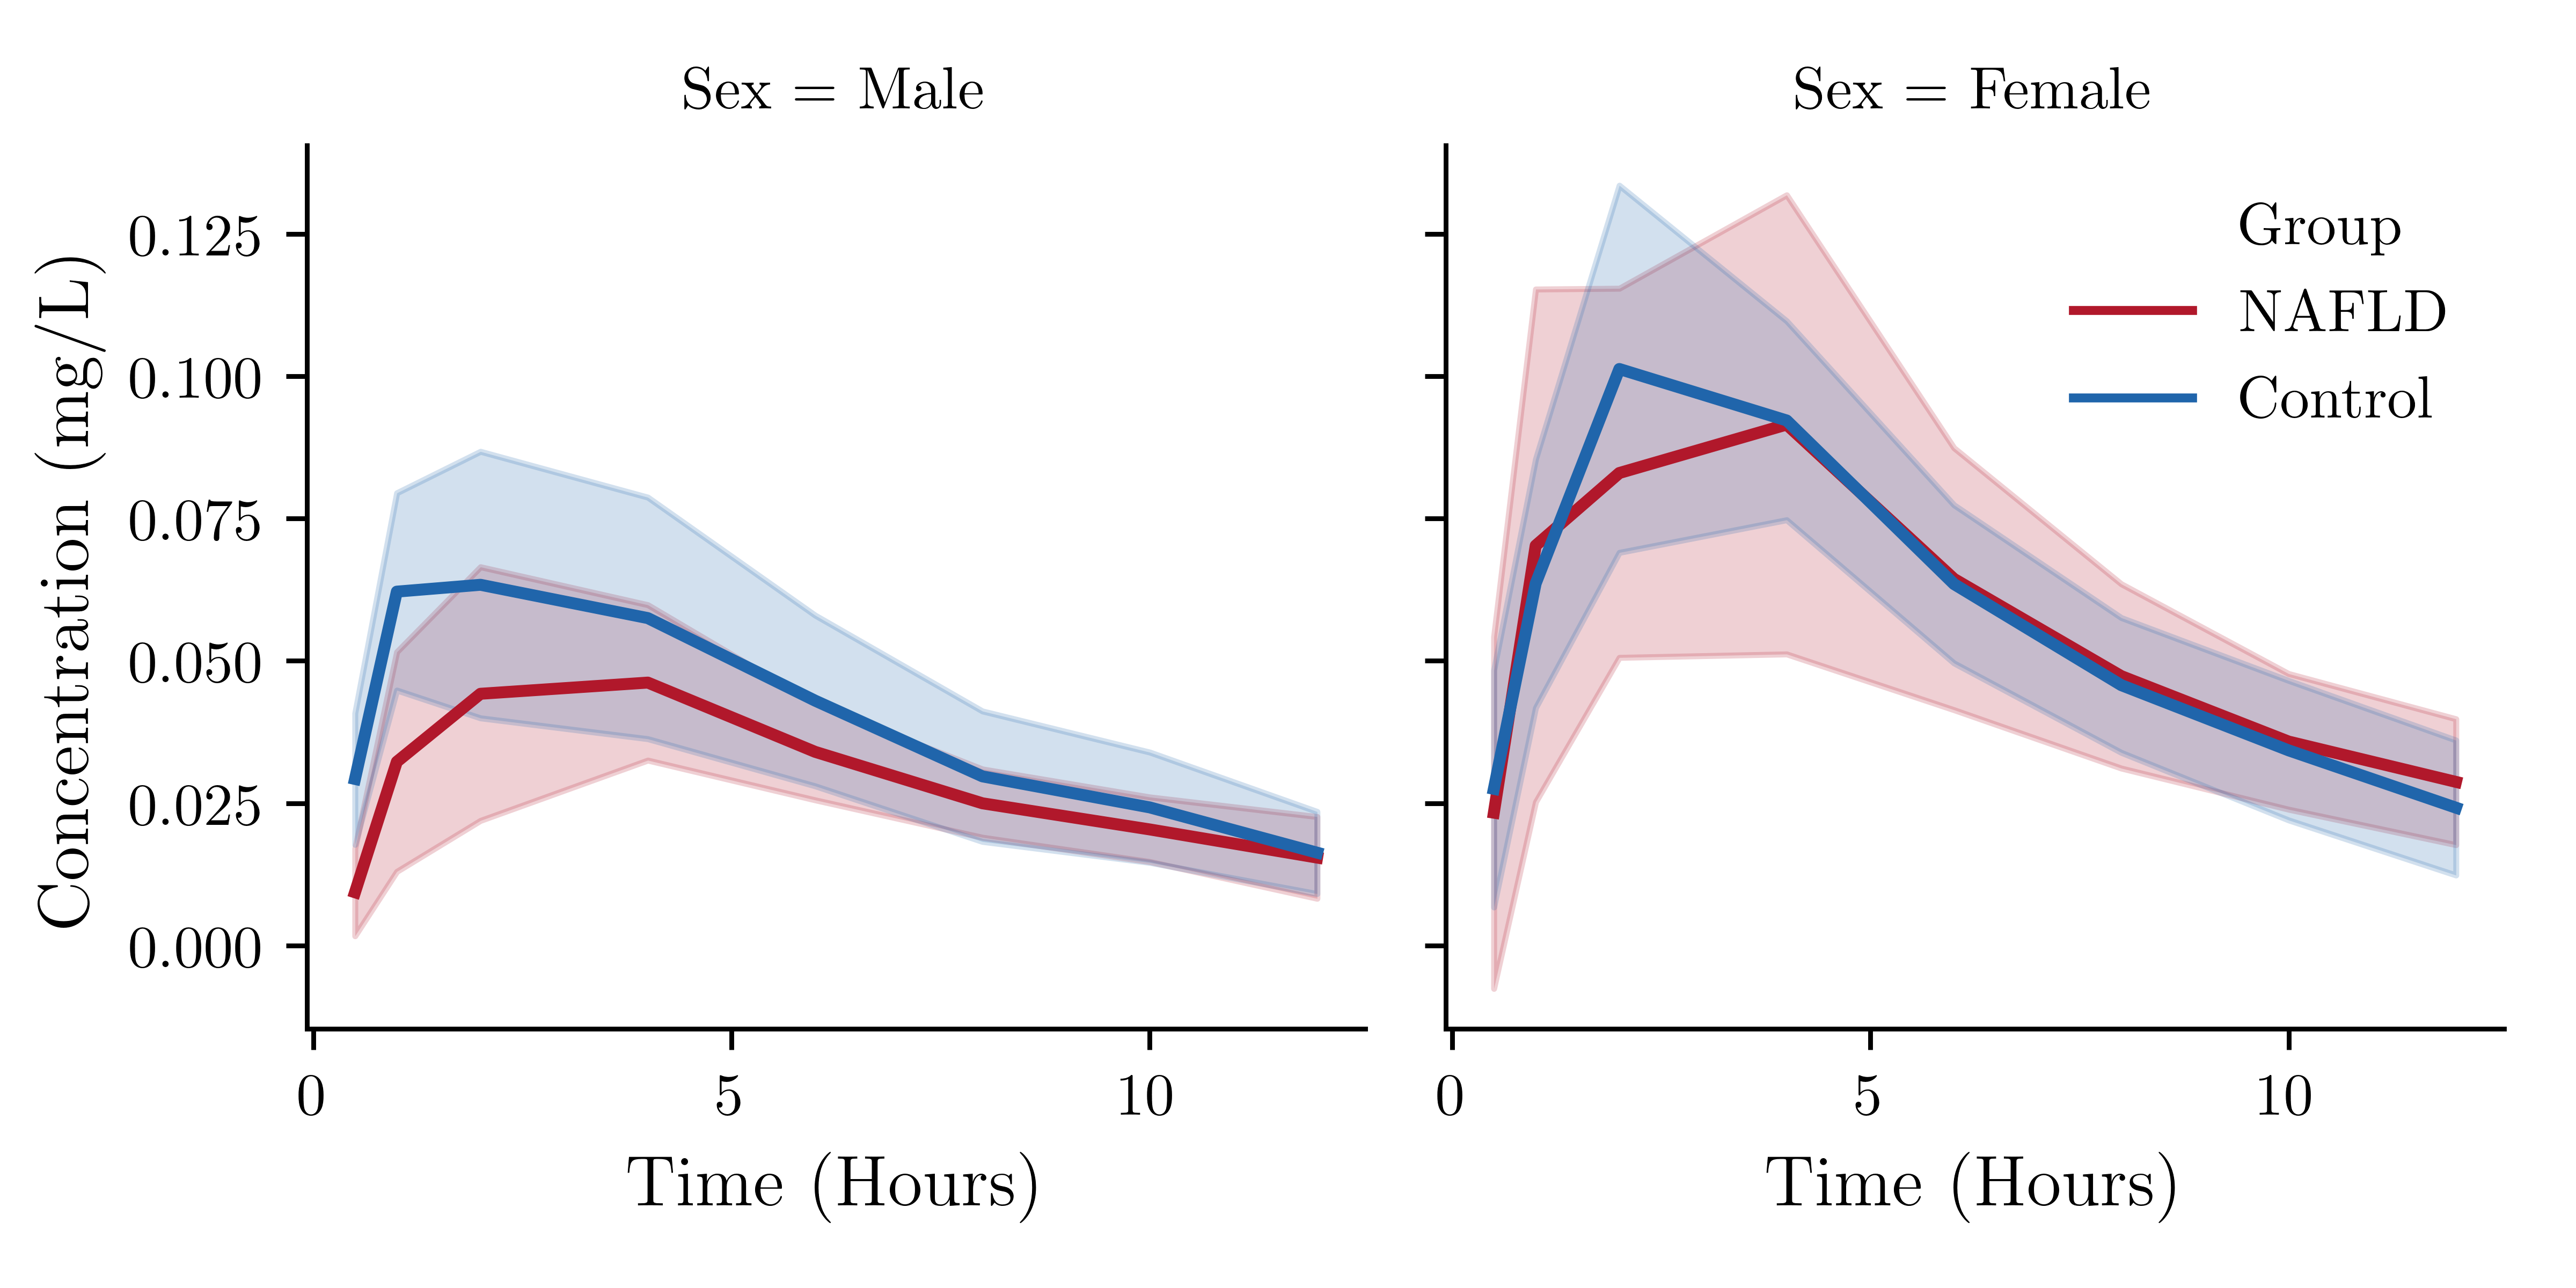
\includegraphics{Figures/data_summary}
	\caption[Concentration profiles for development set]{Concentration profiles for each group of the development set.  Colors indicate group, shaded regions indicate one standard deviation.  There appears to be a noticeable effect of sex on concentration.}
	\label{datasummary}
\end{figure}

\subsubsection{Model 1}
Since the patients in the development set only ingest a single dose of Apixiban on an empty stomach, a simple one compartment model as in \cref{onecompartment_PKPD} is appropriate.  The model will posit that a single set of pharmacokinetic parameters (namely $V$, $k$, and $k_a$) can be used to fit the data.  The model is shown below.

\begin{align}
	V &\sim \operatorname{Log-Normal}(\log(5),0.1) \label{mod_1_V} \\
	k &\sim \operatorname{Half-Cauchy}(0,1) \label{mod_1_k} \\
	k_a &\sim \operatorname{Half-Cauchy}(0,1) \label{mod_1_ka} \\
	\sigma_y &\sim \operatorname{Half-Cauchy}(0,1) \label{mod_1_sigma} \\
	C(t) &= \dfrac{2.5}{V}\dfrac{k_a}{k - k_a}\Big(e^{-k_at} - e^{-kt}\Big) \label{mod_1_C}\\
	\mathbf{y} &\sim \operatorname{Log-Normal}(\log(C(t)), \sigma_y^2) \label{mod_1_y}
\end{align}

\begin{figure}[t!]
	
	\centering
	\begin{tikzpicture}
	
	\node[obs](y){$y_i$};
	\node[latent, above = of y](k){$k$};
	\node[latent, right = of k](ka){$k_a$};
	
	\node[latent, left = of k](V){$V$};
	\node[latent, right = of y, xshift = 1cm](sig){$\sigma_y$};
	
	\node[obs, left = of y](t){$t_i$};
	

	\edge{V}{y};
	\edge{k}{y};
	\edge{ka}{y};
	\edge{sig}{y};
	\edge{t}{y};
	
	\plate{t_y_pairs}{(t)(y)}{$i=1\dots8$};
	
	\end{tikzpicture}
	\caption[Bayes net for first pharmacokinetic model]{Bayes net for the model proposed in \crefrange{mod_1_V}{mod_1_y}.  Shaded discs indicate directly observed variables.}
	\label{model_1}
\end{figure}

The parameter $V$ can be interpreted as the volume of blood (in litres) in the body, and so a log-normal distribution with mean 5 and standard deviation 0.1 is chosen.  Half Cauchy distributions are chosen as weakly informative priors for the pharmacokinetic parameters, as well as the noise. This prior distribution has the the majority of probability centred around 0 but allow for the possibility of large values for the pharmacokinetic parameters.  A log normal distribution is chosen as the likelihood so that the noise in the system does not result in nonphysical simulated data.

It is worth noting that this model ignores the within patient correlation, and is thus not a preferable model with which to do inference.  This is by design, and the complexity of the model will increase as a part of continuous model expansion. 

\subsubsection{Model 2}

The next step of model development will be to create a  pharmacokinetic model in which each patient's pharmacokinetic parameters are estimated as opposed to positing that a single set of pharmacokinetic parameters exist for the population. This is akin to a mixed effects model, in which the pharmacokinetic parameters are random effects.  A hyperprior for the population level mean of the pharmacokinetic parameters will be specified.  The Bayes' net for this model is shown in \cref{model_2}.

By estimating pharmacokinetic parameters for each patient, the within patient correlation is implicitly modelled. The prior distributions for the population means for the pharmacokinetic parameters and blood volume are shown below.  The likelihood and prior for $\sigma_y$ remain the same.

\begin{figure}[h!]
	
	\centering
	\begin{tikzpicture}
	
	\node[obs](y){$y_i$};
	\node[latent, above = of y](k){$k_p$};
	\node[latent, right = of k](ka){$k_{ap}$};
	\node[latent, left = of k](V){$V_p$};
	
	\node[latent, above = of V](mu_V){$\mu_V$};
	\node[latent, above = of k](mu_k){$\mu_k$};
	\node[latent, above = of ka](mu_ka){$\mu_{k_a}$};
	
	
	\node[latent, right = of y, xshift = 1 cm](sig){$\sigma_y$};
	
	\node[obs, left = of y](t){$t_i$};
	
	
	\edge{V}{y};
	\edge{k}{y};
	\edge{ka}{y};
	\edge{sig}{y};
	\edge{t}{y};
	
	\edge{mu_V}{V};
	\edge{mu_k}{k};
	\edge{mu_ka}{ka};
	
	\plate{t_y_pairs}{(t)(y)}{$i=1\dots8$};
	\plate{patient_level}{(V)(k)(ka)(t_y_pairs)}{$p = 1\dots 36$};
	\end{tikzpicture}
	\caption[Bayes net for second pharmacokinetic model]{Bayes net for model 2.  Here, $\sigma_y$, $\mu_V$, $\mu_k$, and $\mu_{k_a}$ are population level parameters, and hence are outside the plates.}
	\label{model_2}
\end{figure}

\begin{align}
	\mu_V &\sim  \operatorname{Normal}(\log(5),1)\\
	V &\sim \operatorname{Log-Normal}(\mu_V, 0.5)\\ \nonumber\\
	\mu_k &\sim \operatorname{Normal}(0,1)\\
	k &\sim \operatorname{Log-Normal}(\mu_k,0.5)\\ \nonumber\\
	\mu_{k_a} &\sim \operatorname{Normal}(0,1)\\
	k &\sim \operatorname{Log-Normal}(\mu_{k_a},0.5)
\end{align}


\subsubsection{Model 3}

The final model extension will be to turn the model presented in the previous section into a full hierarchical regression.  The mean of the pharmacokinetic parameter's population distribution changes with a linear predictor through a link function. This will provide an understanding of how each covariate impacts the metabolism of apixiban.  Shown below are the priors for the new additions.  The likelihood and prior for the noise $ \sigma_y $ remain the same.  The Bayes' net for this model is shown in \cref{model_3}.

\begin{align}
	\sigma_V &\sim \operatorname{Half-Cauchy}(0,1)\\
	\beta_V &\sim \operatorname{Normal}(0,1)\\ 
	\mu_V &= \exp(\mathbf{x}^T\beta_V) \\
	V &\sim \operatorname{Log-Normal}(\mu_V, \sigma_V) \\ \nonumber \\
	%
	\sigma_k &\sim \operatorname{Half-Cauchy}(0,1)\\
	\beta_k &\sim \operatorname{Normal}(0,1)\\ 
	\mu_k &= \exp(\mathbf{x}^T\beta_k) \\
	k &\sim \operatorname{Log-Normal}(\mu_k, \sigma_k) \\ \nonumber \\	
	%
	\sigma_{k_a} &\sim \operatorname{Half-Cauchy}(0,1)\\
	\beta_{k_a} &\sim \operatorname{Normal}(0,1)\\ 
	\mu_{k_a} &= \exp(\mathbf{x}^T\beta_{k_a}) \\
	k_a &\sim \operatorname{Log-Normal}(\mu_{k_a}, \sigma_{k_a}) 
\end{align}


\begin{figure}[t!]
	
	\centering
	\begin{tikzpicture}
	
	\node[obs](y){$y_i$};
	\node[latent, above = of y](k){$k_p$};
	\node[latent, right = of k](ka){$k_{ap}$};
	\node[latent, left = of k](V){$V_p$};
	
	\node[latent, above = of V, yshift = 1cm](b_V){$\beta_V$};
	\node[latent, above = of V, xshift = -0.75cm](sig_V){$\sigma_V$};
	\node[latent, above = of k, yshift = 1cm](b_k){$\beta_k$};
	\node[latent, above = of k, xshift = -0.75cm](sig_k){$\sigma_k$};
	\node[latent, above = of ka, yshift = 1cm](b_ka){$\beta_{k_a}$};
	\node[latent, above = of ka, xshift = -0.75cm](sig_ka){$\sigma_{k_a}$};
	
	
	\node[latent, right = of y, xshift = 1 cm](sig){$\sigma_y$};
	
	\node[obs, left = of y](t){$t_i$};
	
	
	\edge{V}{y};
	\edge{k}{y};
	\edge{ka}{y};
	\edge{sig}{y};
	\edge{t}{y};
	
	\edge{b_V}{V};
	\edge{b_k}{k};
	\edge{b_ka}{ka};
	
	\edge{sig_V}{V};
	\edge{sig_k}{k};
	\edge{sig_ka}{ka};
	
	\plate{t_y_pairs}{(t)(y)}{$i=1\dots8$};
	\plate{patient_level}{(V)(k)(ka)(t_y_pairs)}{$p = 1\dots 36$};
	\end{tikzpicture}
	\caption[Bayes net for the third pharmacokinetic model]{Completely hierarchical regression model.  Not shown here is the explicit dependence of the patient's pharmacokinetic parameters on covariates $\mathbf{x}$.}
	\label{model_3}
\end{figure}

\subsubsection{Other Model Expansions}

Since the patients in the development have ingested a single dose of apixiban, \cref{onecompartment_PKPD} is appropriate.  In practice, patients will have ingested apixiban in the past as part of a daily routine.  This makes \cref{onecompartment_PKPD} inappropriate.  \Cref{onecompartment_PKPD} can be extended to better model daily ingestion of a drug.  Recall that the differential equation governing the dynamics of drug metabolism is
\begin{equation}
	\dfrac{dC}{dt} = \dfrac{D}{V}k_a\exp(-k_a t) - kC \> \quad C(0) = 0 \>.
\end{equation}
To account for multiple doses of size $ D $, this differential equation can be extended through the use of impulse functions.  If the patient takes the drug at times $ \tau_1, \dots , \tau_m $, then the differential equation governing these dynamics can be written as 
\begin{equation} \label{multidose}
\dfrac{dC}{dt} = \dfrac{D}{V}k_a\exp(-k_a t) - kC + \sum_{j=1}^m H(t - \tau_i) k_a \dfrac{D}{V}\exp(-k_a(t-\tau_j)) \>.
\end{equation}
Here, $ H(t) $ is the Heaviside step function.  It can be shown that \cref{multidose} has analytic solution which can be obtained through the use of Laplace Transforms \cite{boyce2012differential}.


\subsection{Adaptive Sampling}



\subsection{Adaptive Control}
